\section{Nested structures}

Now what about situations when one structure is defined inside of another?

\lstinputlisting{patterns/15_structs/5_nested/nested.c}

\dots in this case, both \TT{inner\_struct} fields are to be placed between the a,b and d,e fields of
the \TT{outer\_struct}.

Let's compile (MSVC 2010):

\lstinputlisting[caption=\Optimizing MSVC 2010 /Ob0]{patterns/15_structs/5_nested/nested_msvc.asm}

One curious thing here is that by looking onto this assembly code, we do not even see that
another structure was used inside of it!
Thus, we would say, nested structures are unfolded into \IT{linear} or \IT{one-dimensional} structure.

Of course, if we replace the \TT{struct inner\_struct c;} declaration with \TT{struct inner\_struct *c;} 
(thus making a pointer here) the situation will be quite different.
% FIXME1: нарисовать вложенную структуру и развернутую

\clearpage
\subsection{\olly}
\myindex{\olly}

Let's load the example into \olly and take a look at 
\TT{outer\_struct} in memory:

\begin{figure}[H]
\centering
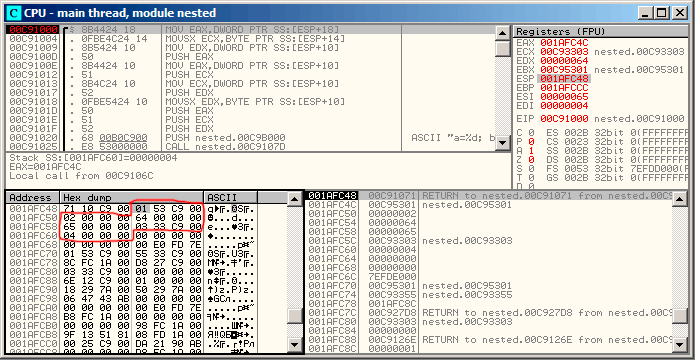
\includegraphics[scale=\FigScale]{patterns/15_structs/5_nested/olly.png}
\caption{\olly: Before \printf execution}
\label{fig:nested_olly}
\end{figure}

That's how the values are located in memory:
\begin{itemize}
\item \IT{(outer\_struct.a)} (byte) 1 + 3 bytes of random garbage;
\item \IT{(outer\_struct.b)} (32-bit word) 2;
\item \IT{(inner\_struct.a)} (32-bit word) 0x64 (100);
\item \IT{(inner\_struct.b)} (32-bit word) 0x65 (101);
\item \IT{(outer\_struct.d)} (byte) 3 + 3 bytes of random garbage;
\item \IT{(outer\_struct.e)} (32-bit word) 4.
\end{itemize}

